\documentclass[12pt,a4paper,twoside]{article}
\usepackage{labor}
\begin{document}

%fill for cover and header creation
\newcommand\laboratorynumber{2}
\title{Abbe-Theorie}
\newcommand\supervisor{Robert Nuster}
\newcommand\groupnumber{42}

\newcommand\participantonelastname{Eisner}
\newcommand\participantonefirstname{Nico}
\newcommand\participantoneid{12214121}
\newcommand\participanttwolastname{Waldl}
\newcommand\participanttwofirstname{Philip}
\newcommand\participanttwoid{12214120}
\author{\participantonelastname \ \& \participanttwolastname}

\newcommand\degreeid{UB 033 678}
\newcommand\semester{23WS}
\date{01.12.2023}

%select correct course title
%\newcommand\coursetitle{Einführung in die \\ physikalischen Messmethoden}
%\newcommand\coursetitle{Laborübungen 1: \\ Mechanik und Wärme}
\newcommand\coursetitle{Laborübungen 2: \\ Elektrizität, Magnetismus, Optik}
%\newcommand\coursetitle{Fortgeschrittenen Praktikum 1: \\ Technische Physik}
%\newcommand\coursetitle{Fortgeschrittenen Praktikum 2: \\ Allgemeine Physik}

%\begin{titlepage}
   \begin{center}
       \begin{figure}[H]
            \begin{minipage}[h]{30mm}
                \centerline{
\includegraphics[height=15mm]{cover_nudes/tugraz.png}}
            \end{minipage}
            \hfill
            \begin{minipage}[h]{30mm}
                \centerline{
\includegraphics[height=15mm]{cover_nudes/nawi_graz.png}}
            \end{minipage}
            \hfill
            \begin{minipage}[h]{30mm}
                \centerline{
\includegraphics[height=15mm]{cover_nudes/uni-graz.png}}
            \end{minipage}
        \end{figure}
        
        \large{\emph{Institut für Experimentalphysik der Technischen Universität Graz \\
        \& Institut für Physik der Universität Graz}} \\
        \vspace{5mm}
        
        {\Huge \textbf{\coursetitle}}
        \vspace{5mm}
        
        {\huge \laboratorynumber: \thetitle}
    \end{center}
    
    \vfill
    
    \begin{table}[H]
        \LARGE
        \centering
        \begin{tabular}{r l}
            Betreuer:       & \supervisor \\
            Gruppennummer:  & \groupnumber \\
            \\
            Name:           & \participantonelastname, \participantonefirstname \\
            Matrikelnummer: & \participantoneid \\
            Name:           & \participanttwolastname, \participanttwofirstname \\
            Matrikelnummer: & \participanttwoid \\
            \\
            Kennzahl:       & \degreeid \\
            Datum:          & \semester \ | \thedate
        \end{tabular}
    \end{table}
    \vspace{4cm}
\end{titlepage}
\clearpage
\setcounter{page}{1}

%\maketitle %short title alternative


\includepdf[pages={1}]{../Deckblätter/Deckblatt_Abbe.pdf}

\tableofcontents
\newpage

\section{Aufgabenstellung} %jo beschreibn wos gmocht host ------------------------------

Der Versuch Abbe-Theorie behandelt, wie aus dem Namen bereits hervorgeht, die gleichnamige Idee von Ernst Abbe, die in erster Linie die von allen Objekten hervorgehenden Beugungseffekte und deren Zusammenhang mit dem Auflösungsverhalten beinhaltet.
Mittels Experiment der Abbe-Theorie soll dies- und einige weitere Eigenschaften dieses Verhaltens nun gezeigt werden.
Die genauen Arbeitsaufträge sehen dabei wie folgt aus:

\begin{itemize}
    \item Vertrautmachen mit dem experimentellen Aufbau
    \item Bestimmung des Auflösungsvermögens einer Linse in Abhängigkeit ihrer numerischen Apertur für
    \begin{itemize}
        \item blaues Licht
        \item rotes Licht
    \end{itemize}
    \item Untersuchung des Zusammenhangs zwischen der Bildauflösung von einem Spaltgitter und der Zahl der transmittierten Beugungsordnungen
    \item  Freies Experimentieren
    \begin{itemize}
        \item Beugungsbild horizontaler Balken
        \item Änderung des Beugungsbild mit dem Abstand der Balken
        \item Grund für Beugungserscheinungen in der Richtung normal zu den Hauptordnungen
        \item Dunkelfeldmikroskopie
        \item Verbindung zu Fourieroptik
    \end{itemize}
\end{itemize}



\section{Voraussetzungen \& Grundlagen} %Grundlagen erklären, Formeln mit erklärung

Das Kapitel Voraussetzungen und Grundlagen wurde basierend auf den literarischen Werken Demtröder \cite{dem2} und dem Script Abbe-Theorie \cite{teachcenter2} verfasst.

\subsection{Auflösungsvermögen und numerische Apertur}

Bei optischen Instrumenten wird das Auflösungsvermögen $\Delta x_{min}$ als der Minimalabstand zwischen zwei Punkte definiert, bei dem das Gerät diese noch als zwei punktförmige Objekte unterscheiden kann.
Dieser Versuch kann mit in dieser Hinsicht mit einem Mikroskop verglichen werden, dessen Auflösungsvermögen wie folgt definiert ist:

\begin{equation}
    \label{eq:Auflösungsvermögen}
    \centerline{$\Delta x_{min} = 0.61\frac{\lambda}{NA}$}
\end{equation}

\noindent
Dabei stellt $\lambda$ die Wellenlänge des verwendeten Lichtes und NA die numerische Apertur des optischen Instrumentes, also grob gesagt dem Öffnungswinkel, durch den das Licht eintreten kann, dar.
Letzteres ist wiederum definiert als:

\begin{equation}
    \label{eq:NA}
    \centerline{$NA = n sin(\alpha)$}
\end{equation}

\noindent
mit n als Brechzahl des Mediums und $\alpha$ dem halben Öffnungswinkel des Lichtkegels. Da n in der Regel (sofern Luft als Medium dient) einen Wert von ziemlich genau 1 annimmt und $\alpha$ als $\tan^{-1}(\frac{R}{g})$ (R ... Linsenradius, g ... Gegenstandsweite) angesehen werden kann (veranschaulicht in Abbildung \ref{fig:NA-Skizze}), lässt sich die Formel für die numerische Apertur auch folgendermaßen umschreiben:

\begin{equation}
    \label{eq:NA-umgeschrieben}
    \centerline{$NA = sin(\tan^{-1}(\frac{R}{g}))$}
\end{equation}

\begin{figure}[H]
    \centering
    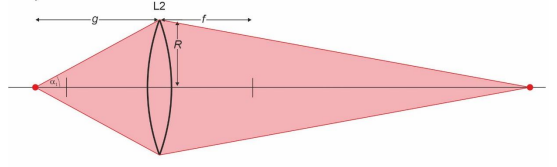
\includegraphics[width=0.5\linewidth]{nudes/NA-Skizze.png}
    \caption{Schematische Darstellung Bestimmmung NA \cite{teachcenter2}}
    \label{fig:NA-Skizze}
\end{figure}


\subsection{Variation der numerischen Apertur}

Der Einfluss des numerischen Apertur kann nur experimentell gezeigt werden, indem man sie variiert. Hierfür bietet es sich an, Linsen mit verschiedenen Durchmessern (Veränderung von R in \ref{eq:NA-umgeschrieben}) zu verwenden, oder der Einsatz einer Lochblende in der hinteren Brennebene der Linse.
Wie genau die numerische Apertur das Auflösungsverhalten beeinflusst wird im folgenden Experiment gezeigt.


\subsection{Abbesche Abbildungstheorie}

Wie im Kapitel Aufgabenstellung bereits einleitend erwähnt, besagt die Abbe Theorie, dass von jedem Objekt Beugungsmaxima hervorgehen und die Auflösung einen Zusammenhang zur Zahl der Beugungsmaxima besitzt.
Wichtig hierbei ist außerdem die Verwendung eines Gitters, dessen Spaltbreite dem halben Spaltabstand entspricht. Somit fehlen fehlen dem Gitter die gradzahligen Beugungsmaxima und am Bild hinter dem Vielfachspalt sind nur die ungradzahligen Maxima erkennbar (wird im Verlauf des Experimentes noch gezeigt).
Mit Hilfe des Tools für die grafische Darstellung solcher Muster von Leifi-Physik \cite{leifi} kann dieses Scenario theoretisch simuliert werden:

\begin{figure}[H]
    \centering
    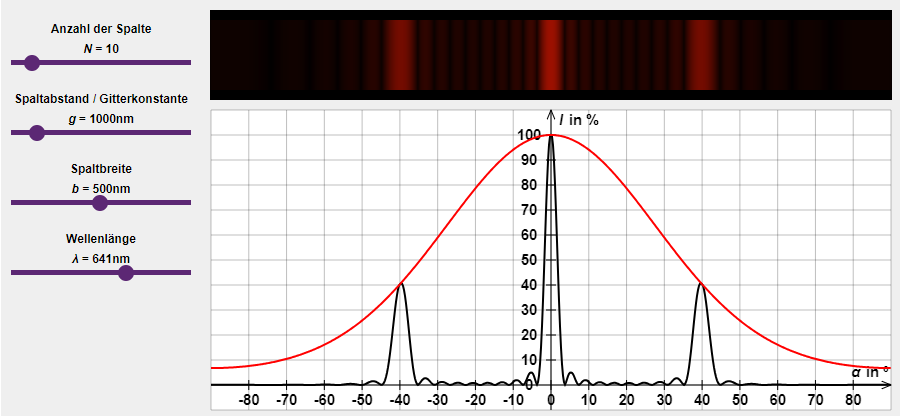
\includegraphics[width=0.4\linewidth]{nudes/VG-Simulation10Nrot.png}
    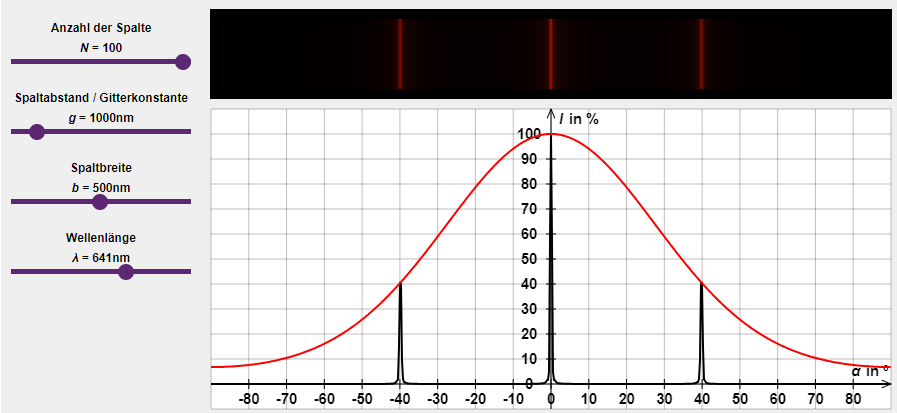
\includegraphics[width=0.4\linewidth]{nudes/VG-Simulation100Nrot.png}
    \caption{Simulation der Maxima einer Gitterbeugung von rotem Licht mit 10/100 Spaltöffnungen}
    \label{fig:SimulationRot}
\end{figure}

\begin{figure}[H]
    \centering
    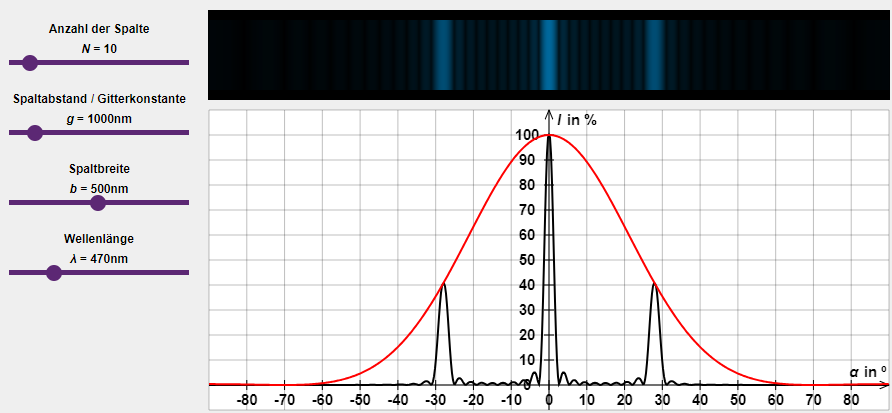
\includegraphics[width=0.4\linewidth]{nudes/VG-Simulation10Nblau.png}
    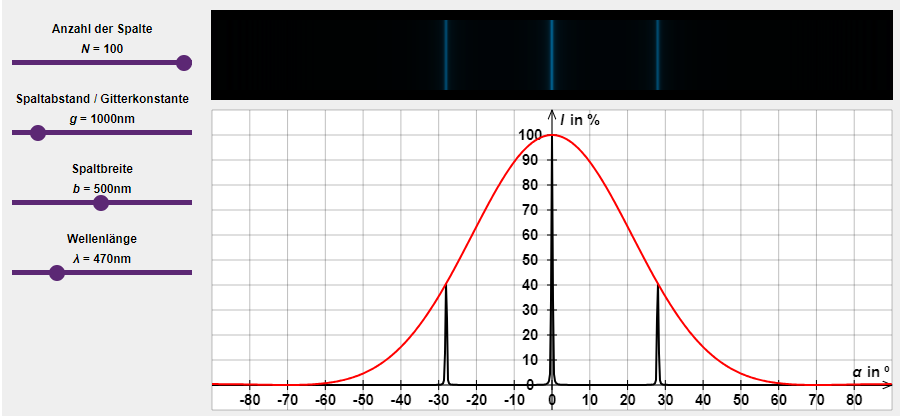
\includegraphics[width=0.4\linewidth]{nudes/VG-Simulation100Nblau.png}
    \caption{Simulation der Maxima einer Gitterbeugung von blauem Licht mit 10/100 Spaltöffnungen}
    \label{fig:SimulationBlau}
\end{figure}


\subsection{Wichtige Zusammenhänge}

Für eine erfolgreiche Auswertung der Daten werden außerdem folgende Zusammenhänge benötigt:

\begin{equation}
    \label{eq:WZ-NA}
    \centerline{Numerische Apertur \\ $NA = \frac{D_{Blende}}{2f_{2}}$ \\ $\Delta NA = \vert \frac{\partial NA}{\partial D_{Blende}} * \Delta D_{Blende} \vert + \vert \frac{\partial NA}{\partial f_{2}} * \Delta f_{2} \vert $}
\end{equation}

\begin{equation}
    \label{eq:WZ-dTheo}
    \centerline{Auflösungsvermögen theoretisch \\ $d_{th} = 0.61\frac{\lambda}{NA}$ \\ $\Delta d_{th} = \vert \frac{\partial d_{th}}{\partial \lambda} * \Delta \lambda \vert + \vert \frac{\partial d_{th}}{\partial NA} * \Delta NA \vert $}
\end{equation}

\begin{equation}
    \label{eq:WZ-fr}
    \centerline{Räumliche Frequenz \\ $f_{R} = 2^{n_{g}^{\frac{n_{E}-1}{6}}}$ \\ $\Delta f_{R} = \vert \frac{\partial f_{R}}{\partial n_{g}} * \Delta n_{g} \vert + \vert \frac{\partial f_{R}}{\partial n_{E}} * \Delta n_{E} \vert $}
\end{equation}

\begin{equation}
    \label{eq:WZ-dExp}
    \centerline{Auflösungsvermögen experimentell \\ $d_{exp} = \frac{1}{f_{R}}$ \\ $\Delta d_{exp} = \vert \frac{\partial d_{exp}}{\partial f_{R}} * \Delta f_{R} \vert$}
\end{equation}


    

\section{Versuchsanordnung} %mit skizze kurz beschreiben ------------------------------

Der Aufbau des Experimentes ist im Grunde sehr simpel. Es besteht aus einer Aluschiene, auf der acht verschiedene Module in einem bestimmten Abstand angebracht sind. 

\begin{figure}[H]
    \centering
    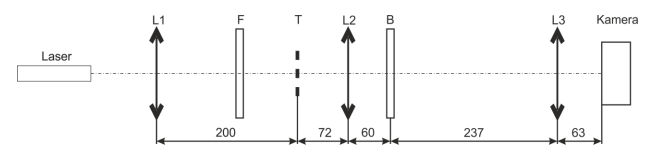
\includegraphics[width=0.8\linewidth]{nudes/VersuchsaufbauTheoretisch.png}
    \caption{Optischer Aufbau des Experiments; L1: f1 = 200mm, F: Filterrad mit roter/blauer LED, Graufilter und freiem
    Durchgang, T: Testobjekt; L2: f2 = 60mm; B: Filterrad mit 2/3/6 mm Lochblenden, einer Irisblende und einer
    Drahtblende, L3(einklappbar): f3 = 50mm. \cite{teachcenter2}}
    \label{fig:VersuchsaufbauTheoretisch}
\end{figure}

\begin{figure}[H]
    \centering
    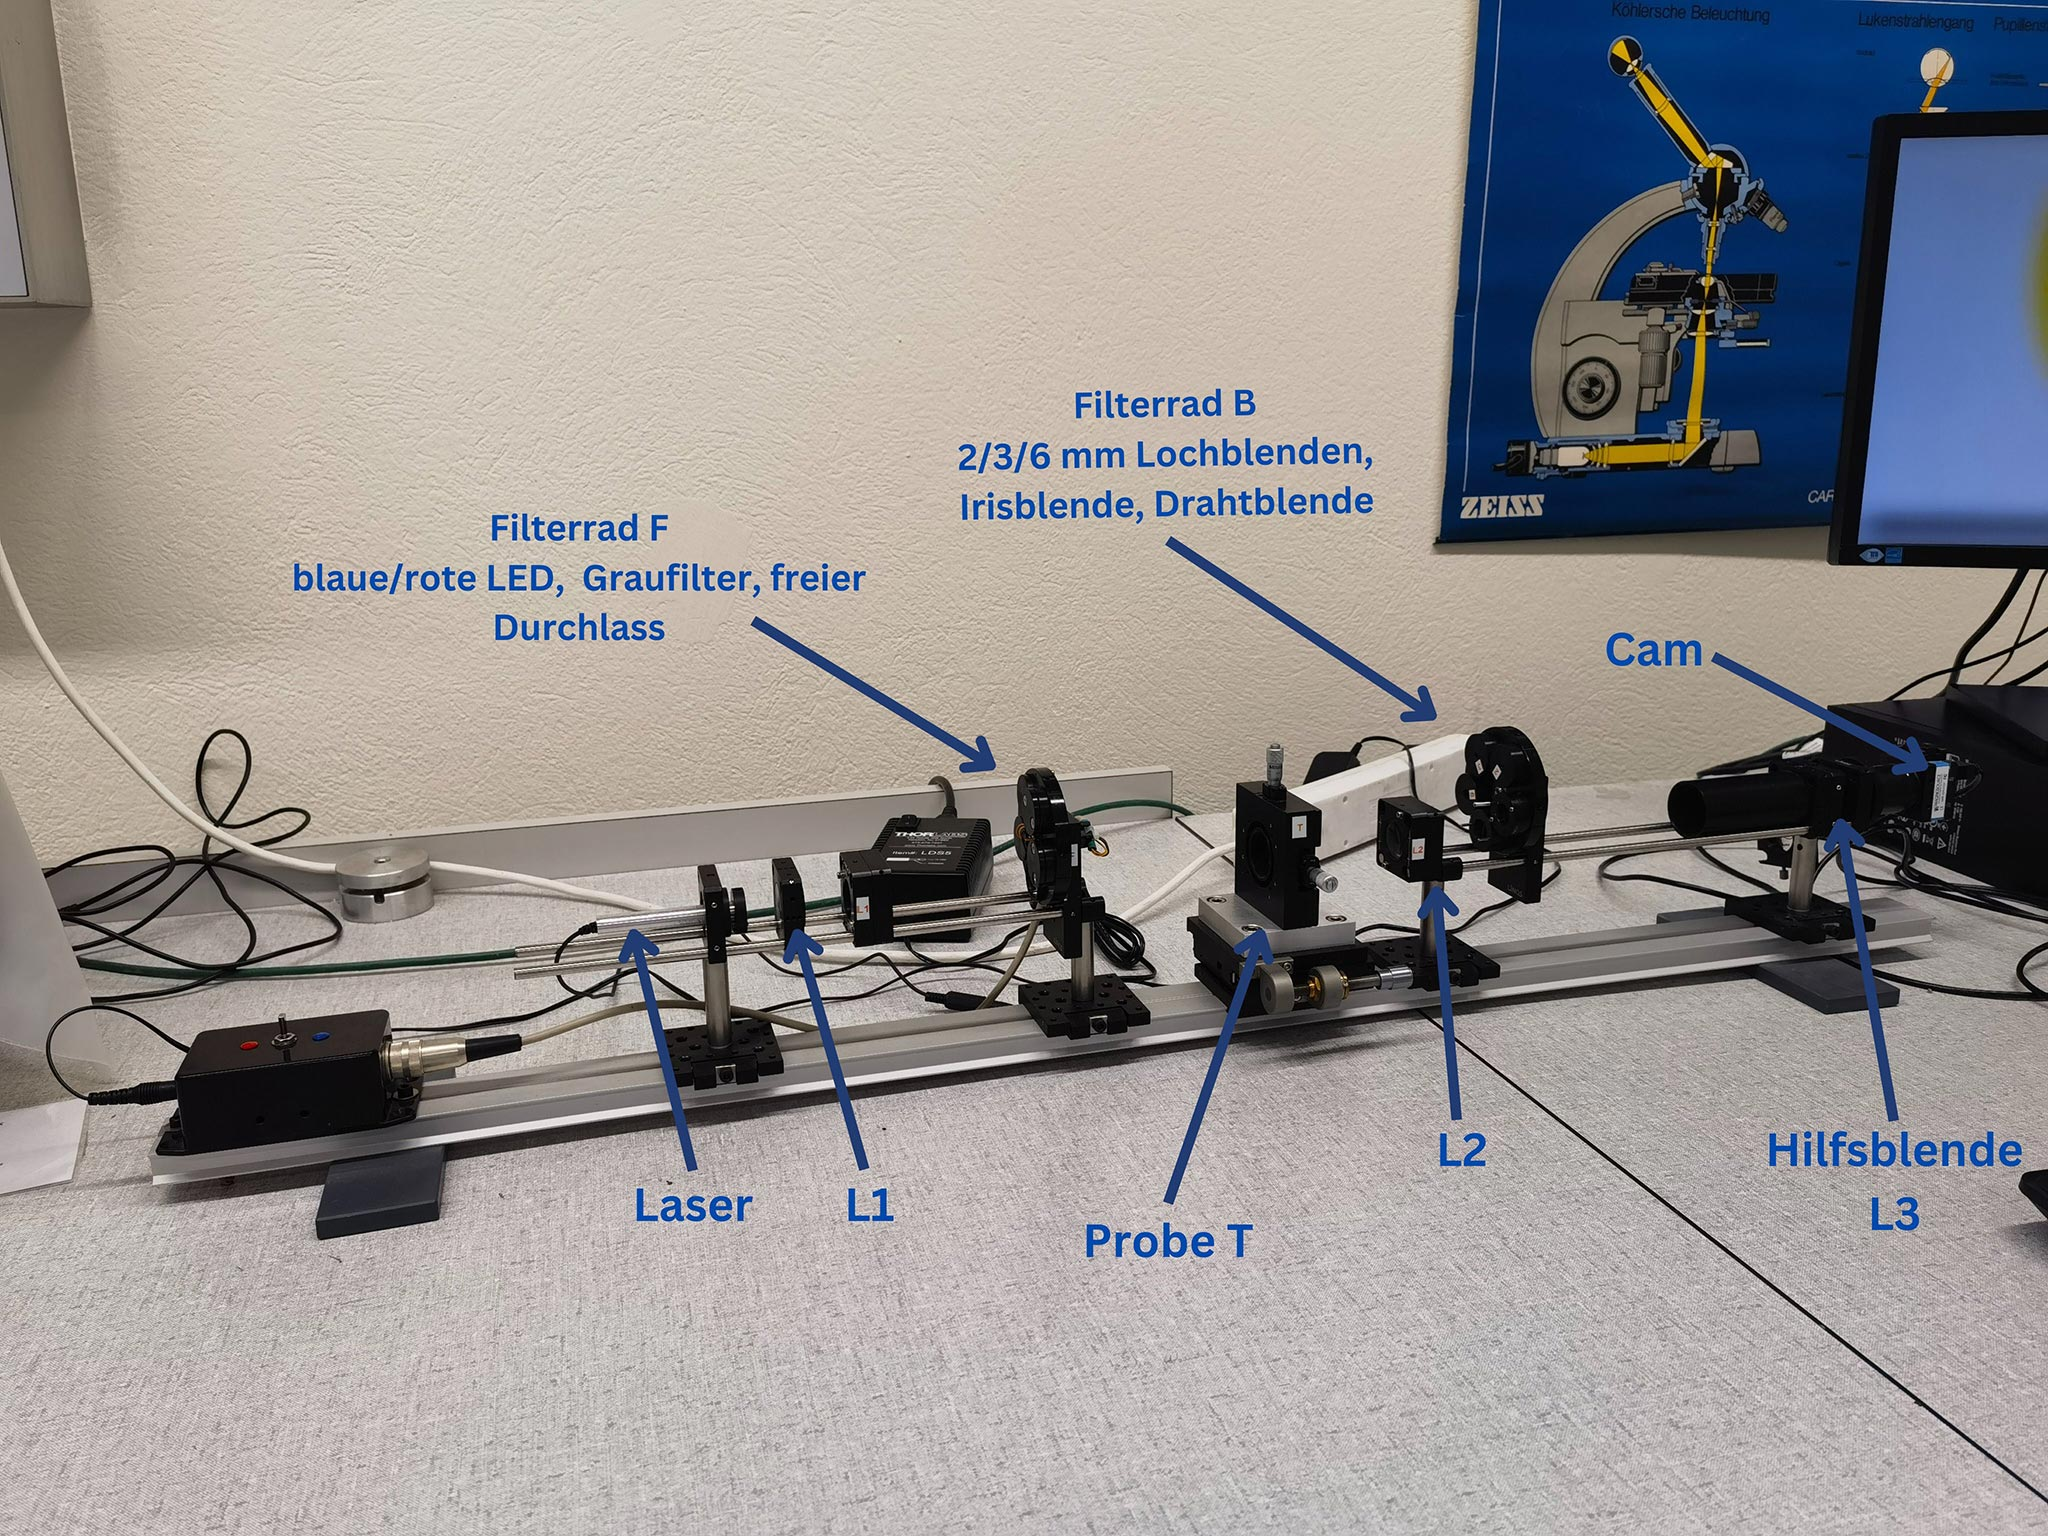
\includegraphics[width=0.7\linewidth]{nudes/VersuchsaufbauIRLbeschriftet.jpg}
    \caption{Versuchsaufbau laut Abbildung \ref{fig:VersuchsaufbauTheoretisch}}
    \label{fig:Versuchsaufbau}
\end{figure}

Die Einzelteile mit Beschreibung sind in folgender Tabelle ersichtlich:

\begin{table}[H]
    \centering
    \caption{Aufbau: Module}
    \label{tab:Aufbau}
    \begin{tabular}{| l | l | l | l |}
        \hline
        Nr.  & Modul & Bezeichnung  & Eigenschaft \\
        \hline
        1 & Laser & Laser & λ= 531,9 nm \\
        2 & Sammellinse 1 & L1 & f1 = 200 mm \\
        3 & Filterrad & F & rote/blauer LED, Graufilter und freier Durchgang \\
        4 & Testobjekt bzw. Probe & T &  \\
        5 & Sammellinse 2 & L2 & f1 = 60 mm \\
        6 & Filterrad & B & 2/3/6 mm Lochblenden, Irisblende und Drahtblende \\
        7 & Sammellinse 3 & L3 & f1 =  50 mm \\
        8 & Kamera & Kamera & Fotosensor mit PC/IC Capture Verbindung \\
        \hline
    \end{tabular}
\end{table}

\noindent
Mit dem Drehrad an der Seite des Testobjektes ist es außerdem möglich, die Schärfe der Probe zu adjustieren. \newline

\noindent
Teil der Vorbereitung war es auch, mögliche Strahlengänge durch diesen Aufbau theoretisch zu zeichnen. Diese sind in nachfolgenden Abbildungen zu sehen.

\begin{figure}[H]
    \centering
    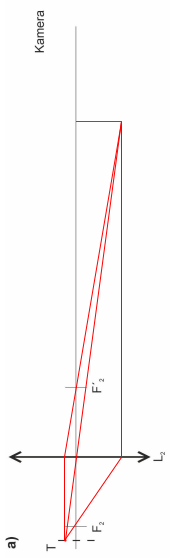
\includegraphics[width=0.3\linewidth, angle=-90]{nudes/Strahlenganga.png}
    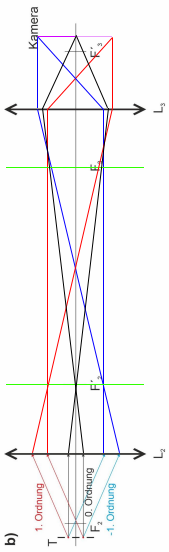
\includegraphics[width=0.3\linewidth, angle=-90]{nudes/Strahlengangb.png}
    \caption{Theoretische Strahlengänge}
    \label{fig:SimulationBlau}
\end{figure}

\section{Geräteliste} %jo holt a listn ------------------------------

    \begin{table}[H]
        \centering
        \caption{Im Versuch verwendete Geräte und Utensilien.}
        \label{tab:geraete}
        \begin{tabular}{| l | l | l | l | l |}
            \hline
            Gerät   & Bezeichnung  & Hersteller  & Eigenschaften  & Unsicherheit \\
            \hline
            Sammellinse & L1 & {n.a} & f1 = 200 mm & 1 mm \\
            Sammellinse & L2 & {n.a} & f1 = 60 mm  & 1 mm \\
            Sammellinse & L3 & {n.a} & f1 = 50 mm  & 1 mm \\
            Laser & Laser & Thorlabs & λ= 531,9 nm & {n.a.} \\
            LED blau & LEDb & Cxxx & λ= 470 nm & 5 nm \\
            LED rot & LEDr & Cxxx & λ= 635 nm & 5 nm \\
            Kamera & Kamera & The Imaging Source & {n.a.} & {n.a.}\\
            Kamera & {n.a.} & The Imaging Source & {n.a.} & {n.a.}\\
            SciDAVis & {n.a.} & Cxxx & {n.a.} & {n.a.} \\
            \hline
        \end{tabular}
    \end{table}


\section{Versuchsdurchführung \& Messergebnisse} %nachvollziehbar und klar dargestellt ------------------------------

Bevor die eigentlichen Messvorgänge starten konnten, war es laut Aufgabe 0 wichtig, sich zuvor mit dem Aufbau und Messinstrumenten vertraut zu machen. 
Der erste Blick fällt dabei auf das Testobjekt des Versuches, dargestellt in folgender Abbildung \ref{fig:Testelement}.

\begin{figure}[H]
    \centering
    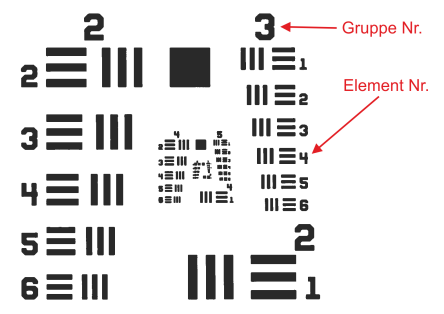
\includegraphics[width=0.6\linewidth]{nudes/Testelement.png}
    \caption{Testelement des Versuches \cite{teachcenter2}}
    \label{fig:Testelement}
\end{figure}

\noindent
Wie sich erkennen lässt, besteht dieses aus mehreren Strichblöcken, die sich aus drei gleichweit voneinander entfernten Linien (je drei horzizontal und drei vertikal ausgerichtet) zusammensetzen.
Zur genauen Beschriftung wurden die Blöcke in Gruppen eingeteilt, welche sich jeweils auf einer Seite der Spirale befinden und durch die großen Zahlen gelabelt sind. Jede Gruppe besteht weiters aus sechs dieser horizontalen- und vertikalen Strichelemente, gekennzeichnet mit einer weiteren Nummerierung.
Mit der nachfolgenden Tabelle \ref{tab:fR-Tabelle} ist jedem Element der Gruppen ein eindeutiger Wert für die räumliche Frequenz $f_{R}$ in 1/mm zugeteilt.

\begin{table}[H]
    \centering
    \caption{Räumliche Frequenz der Balken in 1/mm für die unterschiedlichen Elemente des Testobjektes \cite{teachcenter2}}
    \label{tab:fR-Tabelle}
    \begin{tabular}{|l|llllllllll|}
    \hline
    Element Nr. & \multicolumn{10}{l|}{Gruppen Nr.}                                                                                                                                                                                                                                      \\ \hline
                & \multicolumn{1}{l|}{-2}    & \multicolumn{1}{l|}{-1}    & \multicolumn{1}{l|}{0}    & \multicolumn{1}{l|}{1}    & \multicolumn{1}{l|}{2}    & \multicolumn{1}{l|}{3}     & \multicolumn{1}{l|}{4}     & \multicolumn{1}{l|}{5}    & \multicolumn{1}{l|}{6}     & 7     \\ \hline
    1           & \multicolumn{1}{l|}{0,250} & \multicolumn{1}{l|}{0,500} & \multicolumn{1}{l|}{1,00} & \multicolumn{1}{l|}{2,00} & \multicolumn{1}{l|}{4,00} & \multicolumn{1}{l|}{8,00}  & \multicolumn{1}{l|}{16,00} & \multicolumn{1}{l|}{32,0} & \multicolumn{1}{l|}{64,0}  & 128,0 \\ \hline
    2           & \multicolumn{1}{l|}{0,280} & \multicolumn{1}{l|}{0,561} & \multicolumn{1}{l|}{1,12} & \multicolumn{1}{l|}{2,24} & \multicolumn{1}{l|}{4,49} & \multicolumn{1}{l|}{8,98}  & \multicolumn{1}{l|}{17,95} & \multicolumn{1}{l|}{36,0} & \multicolumn{1}{l|}{71,8}  & 144,0 \\ \hline
    3           & \multicolumn{1}{l|}{0,315} & \multicolumn{1}{l|}{0,630} & \multicolumn{1}{l|}{1,26} & \multicolumn{1}{l|}{2,52} & \multicolumn{1}{l|}{5,04} & \multicolumn{1}{l|}{10,10} & \multicolumn{1}{l|}{20,16} & \multicolumn{1}{l|}{40,3} & \multicolumn{1}{l|}{80,6}  & 161,0 \\ \hline
    4           & \multicolumn{1}{l|}{0,353} & \multicolumn{1}{l|}{0,707} & \multicolumn{1}{l|}{1,41} & \multicolumn{1}{l|}{2,83} & \multicolumn{1}{l|}{5,66} & \multicolumn{1}{l|}{11,30} & \multicolumn{1}{l|}{22,62} & \multicolumn{1}{l|}{45,3} & \multicolumn{1}{l|}{90,5}  & 181,0 \\ \hline
    5           & \multicolumn{1}{l|}{0,397} & \multicolumn{1}{l|}{0,793} & \multicolumn{1}{l|}{1,59} & \multicolumn{1}{l|}{3,17} & \multicolumn{1}{l|}{6,35} & \multicolumn{1}{l|}{12,70} & \multicolumn{1}{l|}{25,39} & \multicolumn{1}{l|}{50,8} & \multicolumn{1}{l|}{102,0} & 203,0 \\ \hline
    6           & \multicolumn{1}{l|}{0,445} & \multicolumn{1}{l|}{0,891} & \multicolumn{1}{l|}{1,78} & \multicolumn{1}{l|}{3,56} & \multicolumn{1}{l|}{7,13} & \multicolumn{1}{l|}{14,30} & \multicolumn{1}{l|}{28,50} & \multicolumn{1}{l|}{57,0} & \multicolumn{1}{l|}{114,0} & 228,0 \\ \hline
\end{tabular}
\end{table}

\noindent
Das Testobjekt wird für spätere Messwerte benötigt. Weiters wurde der Pc gestartet und das Programm IC-Capture gestartet. Nachdem die Kamera verbunden wurde, wurden einige Einstellungen getroffen:

\begin{itemize}
    \item Bildformat: "RGB1280-720" - 3
    \item Histogramm eingeblendet - 2
\end{itemize}

\begin{figure}[H]
    \centering
    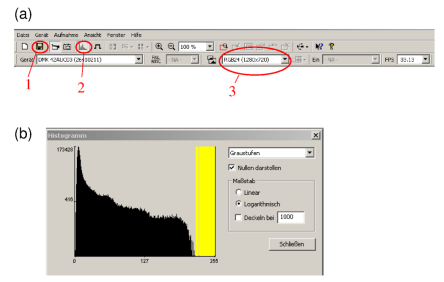
\includegraphics[width=0.5\linewidth]{nudes/IcCaptureSettings.png}
    \caption{a.) IcCapture Einstellungen b.) eingeblendetes Histogramm}
    \label{fig:IcCaptureSettings}
\end{figure}

\noindent
Das Histogramm dient dazu, die Belichtung des aufzunehmenden Bildes zu adjustieren. Hierfür sollte die "Exposure-Time" so eingestellt werden, dass der gelbe Balken rechts gerade noch zu sehen ist, um das Bild optimal zu belichten.


\subsection{Vertrautmachen mit dem Versuch}

Um nun zu Aufgabe 0 zurückzukommen, zu Beginn wurde eine der beiden LEDs (rot oder blau) eingeschaltet und ungehindert durch die Vorrichtung gelassen. Dann wurde die Hilfslinse L3 weggeklappt und die verstellbare Irisblende auf Filterrad B in den Strahlengang gedreht. 
Mit dem kleinen Hebel kann diese geöffnet bzw. geschlossen werden, wobei zunächst für ersteres gesorgt wurde. Am Verschiebeschlitten des Testobkjektes konnte nun auf das Testobjekt fokusiert und dieses somit scharf gestellt werden. 
Mit den Mikrometerschrauben am Verschiebeschlitten des Testelementes konnte nun unterschiedliche Bereiche davon dargestellt werden, wobei die obere Schraube eine Änderung an der x-Achse und die seitliche Schraube eine Änderung auf der y-Achse bewirkt. 
Nun soll ein Bild des Testelementes mit geöffneter- und beinahe geschlossener Irisblende aufgenommen werden. Das Messergebnisse ist in nachfolgenden Abbildungen zu erkennen.

\begin{figure}[H]
    \centering
    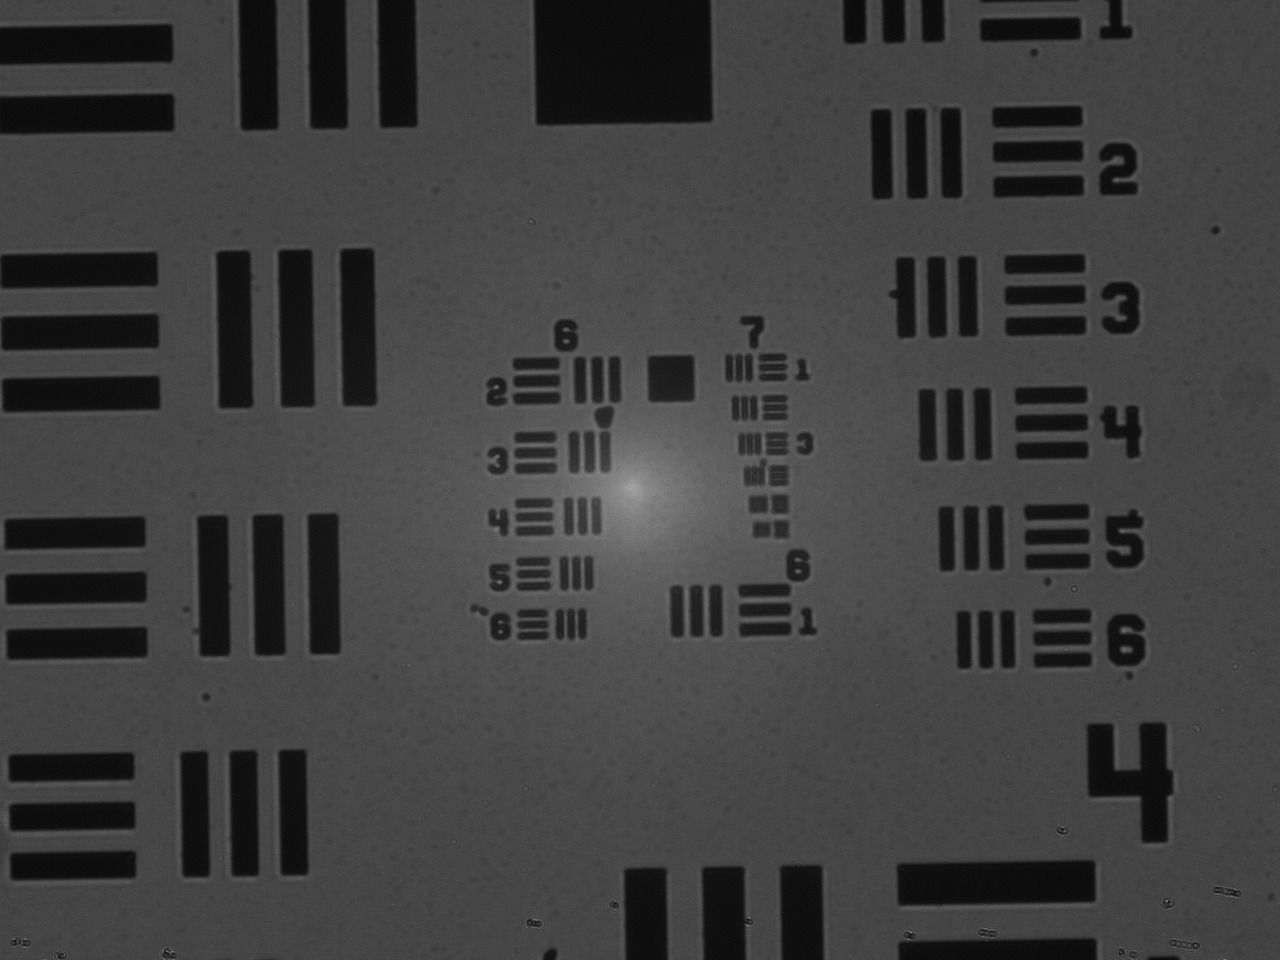
\includegraphics[width=0.4\linewidth]{nudes/AbbeTheorie/Aufgabe 0/scharf-blende-offen.jpg}
    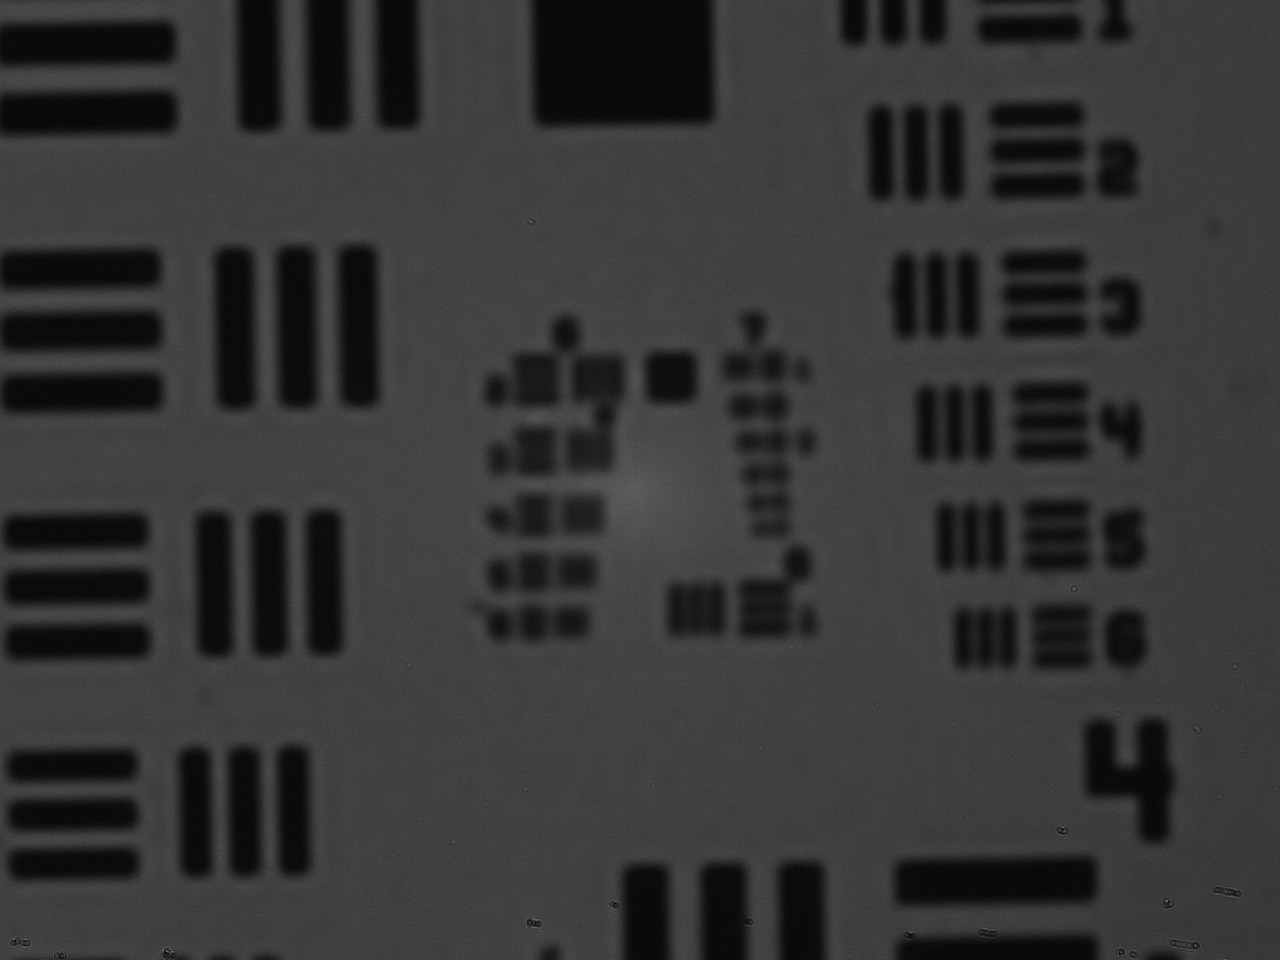
\includegraphics[width=0.4\linewidth]{nudes/AbbeTheorie/Aufgabe 0/scharfgestellt-blende-zu.jpg}
    \caption{Testelement mit geöffneter/fast geschlossener Irisblende}
    \label{fig:Aufgabe0}
\end{figure}


\subsection{Quantitative Bestimmung des Auflösungsvermögens}

Beim nächsten Punkt drehte sich alles um das Auflösungsvermögen. Dieses galt es nämlich in Abhängigkeit der numerischen Apertur für zwei verschiedene Wellenlängen (rotes/blaues Licht) zu bestimmen. 
Hierfür wurde die benötigte LED eingeschaltet und in den Strahlengang eingebracht. Mit Hilfe der drei verschiedenen Lochblenden am Filterrad B kann die numerische Apertur gemäß Formel \ref{eq:NA-umgeschrieben} (Änderung des Radius R) variiert werden. \newline

\noindent
Zu beachten gibt es einen Abbildungsfehler, der durch die LED-Linse entsteht und einen weißen Punkt am Bild erscheinen lässt. Durch verschieben des Testelement mittels der beiden Drehschrauben soll dieser Punkt an einen für die Messung unwichtigen Ort (am Besten die Mitte der Spirale) verschoben werden. \newline

\noindent
Nun sollen die Bilder für jede Lochblende untersucht werden. Dabei wird jenes Balkenelement (horizontal und vertikal) bestimmt, welches nichtmehr erkennbar ist. Dieses Element gilt es in der Tabelle \ref{tab:fR-Tabelle} ausfindig zu machen und die daraus folgenden Werte zu notieren.
Bei dieser Herangehensweiße gibt es einen Ermessensspielraum bei der Entscheidung, ob die Balken noch erkennbar sind oder nicht. Dieser Spielraum stellt für die spätere Auswertung die Unsicherheit dar.

\begin{table}[H]
    \centering
    \caption{Messung des Auflösungsvermögens für rotes Licht}
    \label{tab:BerechnungenLeerlauf}
    \begin{tabular}{| l | l | l | l | l | l |}
        \hline
        Nr. & Blende & Gruppe & Element & \multicolumn{2}{|c|}{Unsicherheit} \\
        \hline
        1 & 2 & 5 & 4 & 5/3 & 5/5 \\
        2 & 3 & 6 & 1 & 5/7 & 6/2 \\
        3 & 6 & 6 & 5 & 6/4 & 6/6 \\
        \hline
    \end{tabular}
\end{table}

\begin{table}[H]
    \centering
    \caption{Messung des Auflösungsvermögens für blaues Licht}
    \label{tab:BerechnungenLeerlauf}
    \begin{tabular}{| l | l | l | l | l | l |}
        \hline
        Nr. & Blende & Gruppe & Element & \multicolumn{2}{|c|}{Unsicherheit} \\
        \hline
        1 & 2 & 5 & 5 & 5/4 & 5/6 \\
        2 & 3 & 6 & 3 & 6/2 & 6/4 \\
        3 & 6 & 7 & 1 & 6/6 & 6/2 \\
        \hline
    \end{tabular}
\end{table}




\subsection{Zusammenhang Auflösung Spaltgitterbildes und Anzahl Beugungsordnungen}
\subsection{Freies Experimentieren}


\section{Auswertung und Unsicherheitsanalyse} %Nicht nur zahlen angeben ------------------------------

In der Auswertung werden zur erhöhten Genauigkeit durchgehend ungerundete Werte bis zu den Endergebnissen verwendet und nur zur Darstellung gerundet. \\
Zur Berechnung der Unsicherheiten wird, wenn nicht anders angegeben, die Größtunsicherheitsmethode verwendet.


\subsection{Quantitative Bestimmung des Auflösungsvermögens}
\subsection{Zusammenhang Auflösung Spaltgitterbildes und Anzahl Beugungsordnungen}
\subsection{Freies Experimentieren}



\section{Diskussion} %diskussion der Unsicherheiten und Ergebnisse und evtl. verlgeich mit Literatur ------------------------------

\subsection{Vertrautmachen mit dem Versuch}
\subsection{Quantitative Bestimmung des Auflösungsvermögens}
\subsection{Zusammenhang Auflösung Spaltgitterbildes und Anzahl Beugungsordnungen}
\subsection{Freies Experimentieren}



\section{Zusammenfassung} %klare, übersichtliche vollständige beantwortung der Aufgabenstellung ------------------------------

\subsection{Quantitative Bestimmung des Auflösungsvermögens}
\subsection{Zusammenhang Auflösung Spaltgitterbildes und Anzahl Beugungsordnungen}
\subsection{Freies Experimentieren}




\printbibliography[heading=bibintoc]
\end{document}
